\chapter{(E) Processi stocastici}

\section{(E-0) Sviluppo del processo lognormale a variabile stocastica binaria}
\lipsum[1-3]

\section{(E-1) Convergenza del processo binario al processo lognormale gaussiano}

\begin{figure}[t]
    \centering
    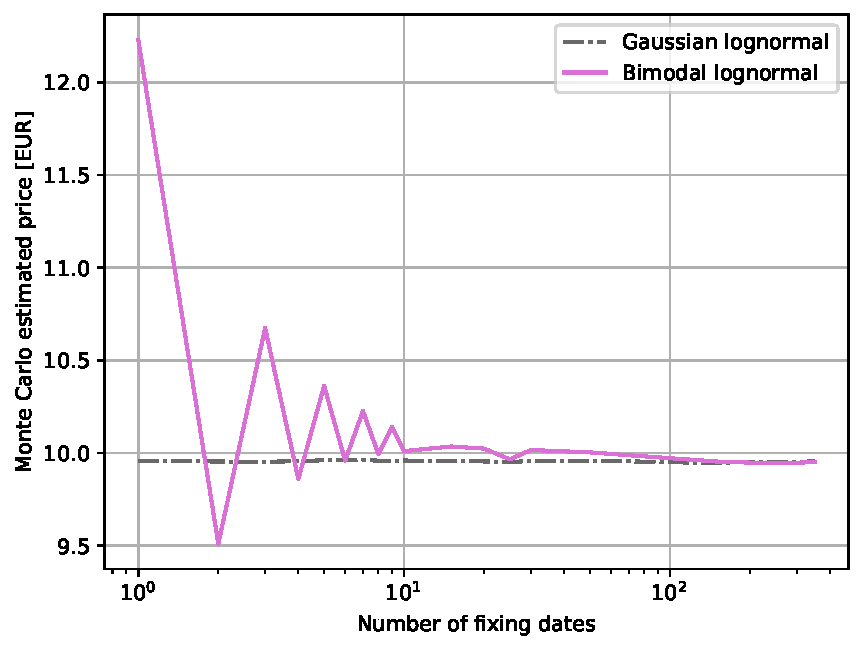
\includegraphics[scale=0.5]{graphs/OptionPriceBimodal_PriceVsM.pdf}
    \caption{Prezzo stimato dell'opzione \textit{performance corridor} tramite lo schema lognormale esatto sfruttando variabili pseudocasuali bimodali (\textit{rosso}) e gaussiane di media nulla e varianza unitaria (\textit{nero, tratteggiato}.}
    \label{fig:bimodal}
\end{figure}

\lipsum[1-3]